\section{Procedimento su HEC-HMS}
Dopo aver ottenuto la funzione della LSPP per il proprio tempo di ritorno, è possibile studiare l'analisi idrologica su HEC-HMS.\\
Per fare ciò, è necessario creare un modello idrologico per ogni bacino, in modo da immettere in input i valori pluviometrici calcolati precedentemente.\\
Il \textit{modello idrologico} è una semplificazione del fenomeno reale (nel nostro caso la trasformazione degli afflussi in deflussi).\\
Il modello idrologico, affinché possa essere soggetto della simulazione, deve avere i seguenti parametri:
\begin{itemize}
    \item bacino idrologico: indica la struttura del bacino, comprendente gli eventuali sottobacini o particolari elementi idraulici;
    \item modello meteorologico: sintetizza le caratteristiche pluviometriche dell'evento meteorologico, come per esempio i bacini interessati o gli effetti ambientali del vento e dell'evapotraspirazione;
    \item specifiche di controllo: possiedono le caratteristiche generali della simulazione da effettuare;
    \item serie di dati temporali: rappresentano i valori (noti) che è possibile introdurre nel modello meteorologico, come per esempio valori pluviometrici o di deflusso.
\end{itemize}
 Ulteriori proprietà, come per esempio il modello digitale del terreno, possono essere introdotti successivamente nel software.\\
 Come anticipato precedentemente, in questa relazione si andrà a studiare la risposta idrologica di due bacini, quindi risulta necessario creare due modelli di calcolo.

\subsection{Creare e calibrare il modello idrologico}
Al fine di creare un modello idrologico, e conseguentemente calibrarlo, si è scelto di studiare i bacini simulando l'evento eccezionale di Vaia del 2018.\\
In questo modo, avendo a disposizione valori certi di afflussi e deflussi, è possibile paragonare la risposta di output dal bacino che il programma calcola, con quella effettivamente misurata.\\
Al fine di cominciare l'analisi in HEC-HMS, è necessario introdurre nel software i parametri precedentemente elencati, riferiti alla tempesta Vaia:
\begin{itemize}
    \item bacino idrologico: sono stati introdotti i file raster dei bacini (\ref{bacino_boite} e \ref{bacino_piave}) ed i valori di primo tentativo di CN e Lag time di piena (rispettivamente 35 e 270 minuti);
    \item modello meteorologico: è stata specificata la sola natura pluviometrica dell'evento, e quali bacini meteorologici incide;
    \item specifiche di controllo: si è definito il periodo interessato, che in questo caso va dal 27 ottobre 2018 al 1 novembre 2018;
    \item serie di dati temporali: sono stati introdotti i valori pluviometrici analizzati dai pluviometri di ogni sottobacino ed i valori di deflusso misurati dagli idrometri alla sezione di chiusura.
\end{itemize}

Dopo aver lanciato la simulazione, il cui procedimento è ampliamente riportato nel manuale ufficiale \cite{manual_hec_hms}, è possibile studiare il grafico afflussi-deflussi che il programma restituisce.\\
Il grafico riferito all'elemento in uscita dal bacino, sia questo un tratto di fiume o un punto di confluenza, possiede un solo istogramma di pioggia, ma due linee di deflusso: una riferita all'evento reale (misurato) ed una calcolata secondo i parametri di primo tentativo introdotti all'inizio.\\
Molto probabilmente, può capitare che le linee di deflusso non coincidano reciprocamente in modo sufficientemente buono; per questo motivo, risulta essenziale svolgere la \textit{calibrazione del bacino}.\\
Il processo di calibrazione del modello consiste nell'indicare al programma quali parametri del bacino andare a modificare (come per esempio il CN o il lag time), in modo che la curva del deflusso calcolato possa coincidere nel modo più ottimale possibile con quella osservata.\\
Dopo aver svolto il processo di calibrazione, è possibile introdurre i parametri ottimali che il programma restituisce nel riquadro inerente alle caratteristiche del bacino; in questo modo si è a conoscenza delle caratteristiche (temporali o fisiche) che meglio approssimano quelle reali.
\begin{figure}[H]\centering
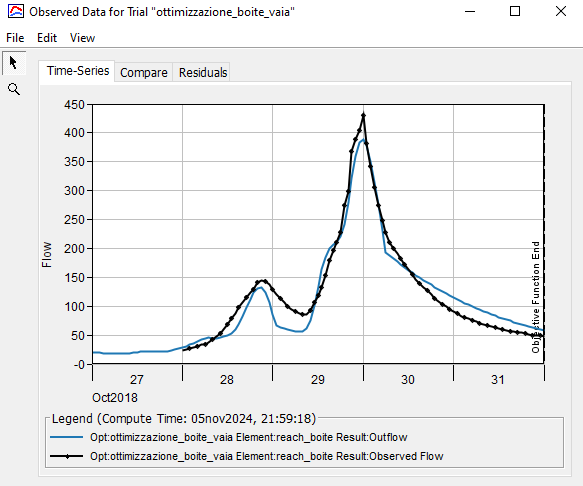
\includegraphics[scale=1]{immagini/ottim_boite.PNG}
\caption{Grafico afflussi-deflussi ottimizzato del bacino del Boite, riferito all'evento della tempesta Vaia.}
    \label{ottim_boite}    
\end{figure}

\begin{figure}[H]\centering
    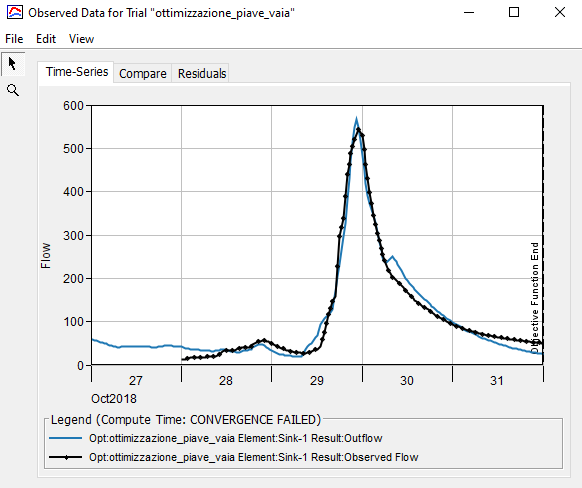
\includegraphics[scale=1]{immagini/ottim_piave.PNG}
    \caption{Grafico afflussi-deflussi ottimizzato del bacino del Piave, riferito all'evento della tempesta Vaia.}
        \label{ottim_piave}    
\end{figure}